\documentclass[11pt]{article}
%%% Preamble for Pomona Linguistics Paper Template %%%

%%%%%%%%%%%%%%%%%%%%%%%%%%%%
%% Document Setup & Layout
%%%%%%%%%%%%%%%%%%%%%%%%%%%%
\usepackage[utf8]{inputenc}
\usepackage[margin=1in]{geometry}
\usepackage{titlesec}
\usepackage[parfill]{parskip}
\setlength{\parindent}{20pt}
\usepackage{setspace}
\singlespacing %\doublespacing 
\sloppy
%%%%%%%%%%%%%%%%%%%%%%%%%%%%
%% Math & Logic
%%%%%%%%%%%%%%%%%%%%%%%%%%%%

\usepackage{amsmath, amssymb, amsfonts, amsthm}
\usepackage{pifont}
\newcommand{\cmark}{\ding{51}}%
\newcommand{\xmark}{\ding{55}}%
\theoremstyle{definition}
\newtheorem{definition}{Definition}[section]
\newcommand{\kuo}[1]{(\ref{#1})}
\newcommand{\forth}[1]{(\citeauthor{#1} (forthcoming)}
\usepackage{expex}

%%%%%%%%%%%%%%%%%%%%%%%%%%%%
%% Fonts & Symbols
%%%%%%%%%%%%%%%%%%%%%%%%%%%%

%\usepackage{fourier}
\usepackage{libertine}
\usepackage{tipa}         % For IPA symbols
\usepackage{textgreek}    % Greek outside math mode
\usepackage{ulem}         % Underline/strikeout


%%%%%%%%%%%%%%%%%%%%%%%%%%%%
%% Tables & Figures
%%%%%%%%%%%%%%%%%%%%%%%%%%%%

\usepackage{booktabs, caption, makecell, array, tabularx, multirow, multicol}
\usepackage{adjustbox}
\usepackage{float}
\usepackage{graphicx}
\usepackage{subcaption}
\usepackage[table]{xcolor}




%%%%%%%%%%%%%%%%%%%%%%%%%%%%
%% Trees & Diagrams
%%%%%%%%%%%%%%%%%%%%%%%%%%%%
\usepackage[linguistics]{forest}
%\forestset{
%  asr/.style={
%    for tree={
%      align=center,
%      parent anchor=south,
%      s sep=4mm,
%      l sep=6mm
%    }
%  },
%  strike/.style={
%    edge label={
%      node[midway, sloped, rotate=90] {=}
%    }
%  }
%}
\usepackage{qtree}

% Arrows and positioning
\usepackage{tikz}
\usetikzlibrary{arrows, arrows.meta, positioning, matrix, tikzmark}
\usepackage{pstricks, pst-node}

% TikZ node circle command
\newcommand{\circled}[1]{\begin{tikzpicture}[baseline=(word.base)]
\node[draw, rounded corners, text height=8pt, text depth=2pt, inner sep=2pt,
outer sep=0pt, use as bounding box] (word) {#1};
\end{tikzpicture}
}
\tikzset{state/.style={circle, draw, minimum size=20pt, inner sep=5pt}}

%%%%%%%%%%%%%%%%%%%%%%%%%%%%
%% Algorithms
%%%%%%%%%%%%%%%%%%%%%%%%%%%%

\usepackage{algorithm}
\usepackage{algpseudocode}
\algrenewcommand\algorithmiccomment[1]{\hfill{\footnotesize\textit{// #1}}}
%\algrenewcommand\algorithmiccomment[1]{\hfill$\triangleright$~
%{\footnotesize\textit{#1}}}


%%%%%%%%%%%%%%%%%%%%%%%%%%%%
%% Linguistics & Glossing
%%%%%%%%%%%%%%%%%%%%%%%%%%%%

\usepackage{leipzig}
\usepackage{expex}
\usepackage{gb4e}
\noautomath % needed for gb4e in some cases
\usepackage{phonrule} % SPE-style rules
\usepackage{marvosym}
%%%%%%%%%%%%%%%%%%%%%%%%%%%%
%% Text & Misc
%%%%%%%%%%%%%%%%%%%%%%%%%%%%

\usepackage{enumitem}
\setlist[itemize]{itemsep=1mm, parsep=0pt}
\usepackage{ragged2e}
\usepackage{stackengine}
\usepackage{verbatim}
\usepackage{todonotes}
\usepackage{color, soul}
\usepackage{metalogo}  % for XeLaTeX logo, etc.

\usepackage{bm} % for bold math symbols
%\usepackage{wasysym}
%%%%%%%%%%%%%%%%%%%%%%%%%%%%
%% Hyperlinks & Citations
%%%%%%%%%%%%%%%%%%%%%%%%%%%%

\usepackage[
  colorlinks = true,
  linkcolor = blue,
  urlcolor  = blue,
  citecolor = blue,
  anchorcolor = blue
]{hyperref}
\usepackage{natbib}

%%%%%%%%%%%%%%%%%%%%%%%%%%%%
%% Shortcuts & Tweaks
%%%%%%%%%%%%%%%%%%%%%%%%%%%%

\usepackage{xspace}
\xspaceaddexceptions{]\}}

% Replace default emptyset with nicer one

\makeatletter
\def\maketitle{%
  \begin{center}
    {\Large \bfseries \color{black} \@title \par}

%    {\normalsize \@author \par}

%    {\small \@date \par}
  \end{center}
}
\makeatother

\let\oldemptyset\emptyset
\let\emptyset\varnothing
\newcommand{\nothing}{$\emptyset$}

% Leipzig glossing again (required by some documents)
\RequirePackage{leipzig}

%%%%%%%%%%%%%%%%%%%%%%%%%%%%%%%%%%%%%%%%%%%%%%%%
%% END of preamble
%%%%%%%%%%%%%%%%%%%%%%%%%%%%%%%%%%%%%%%%%%%%%%%%

\title{Register and Representation of Shanghai Chinese}
\begin{document}
\maketitle

Shanghainese (Shanghai Chinese) is a variety of Wu Chinese spoken in Shanghai. 
It has long served as an important case for illustrating the interaction 
between tone and segmental features. Despite being relatively well studied, 
Shanghainese still presents a number of long-standing, unresolved debates 
concerning the behavior and representation of its tones. One of the central 
debates concerns the representation of register. 
\citet{yip1980}. Murmur is a phonetic manifestation of register: in addition to 
the usual pitch lowering, it is accompanied by breathy voice. Previous research 
differs on where register should be located within tonal geometry. Two 
competing views exist: one treats register as a feature that dominates at the 
word level, while the other treats it as a feature associated with the voicing 
node of a segment.

This paper is motivated by that question and has two goals. First, we provide a 
more rigorous mathematical framework to model these two approaches, allowing 
for a precise comparison of their predictive power and expressiveness. 
Second, we employ computational methods to learn the tonotactics of 
Shanghainese under both representational assumptions, comparing the learning 
results to evaluate their relative outcomes.


\section{Shanghai Tonology}

Shanghai Chinese has five tones (T1–T5). Previous research has shown a variety 
of transcription systems for these tones, whether using the five-point scale 
notation \citep{chao1930system} or more phonologically oriented representations 
indicating tonal height \citep{yip1980}. These systems largely converge on the 
overall contour shapes but differ in the precise pitch value of tonal onsets 
and offsets. 

\begin{table}[htbp]
	\centering
	\begin{tabular}{cccccc}
		\toprule
		Tone & \citet{MFCdatabase} & \citet{xu1988description} & \citet{duanmu1999metrical} &  ?  & \citet{zee1979tones} \\ \midrule
		 T1  &         53          &            53             &            /HL/            & /H/ &          HL          \\
		 T2  &         34          &            24             &            /LH/            & /L/ &         /MM/         \\
		 T3  &         23          &            13             &            /LH/            & /L/ &         /ML/         \\
		 T4  &          5          &         \emph{55}         &            /LH/            & /L/ &         /H/          \\
		 T5  &         12          &         \emph{13}         &            /LH/            & /L/ &         /LM/         \\ \bottomrule
	\end{tabular}
	\caption{Transcriptions of Shanghai tones across sources}
	\label{tab:transcript}
\end{table}


The Shanghai tonal system is regarded as a \textit{complex} system. Unlike 
Mandarin, in which tonal contrasts are primarily distinguished by pitch, tonal 
recognition in Shanghai Chinese also relies on \textit{register }and vowel 
\textit{length} \citep{zhu+2015tone}. As shown in Figure~\ref{tab:shanghai}, 
there are two registers \textsc{[upper]} (discussed in detail in the next 
section), and two major syllable types: slack syllables and checked syllables 
(those closed by a glottal stop). The following section will focus on previous 
studies of register and length contrasts in Shanghai tonology.

\begin{table}[h!]
	\centering
	\begin{tabular}{ccccccccc}
		\toprule
		\multirow{2}{*}{\textbf{Register}} & \multirow{2}{*}{\textbf{Tone}} 
		& \multicolumn{3}{c}{Slack syllable} & & \multicolumn{3}{c}{Checked syllable} \\ 
		\cmidrule{3-5}\cmidrule{7-9}
		&  & \textbf{TV(\ng)} & \textbf{DV(\ng)} & \textbf{SV(\ng)} & & \textbf{TV\textglotstop} & \textbf{DV\textglotstop} & \textbf{SV\textglotstop} \\
		\midrule
		\multirow{3}{*}{\textbf{+upper}} 
		& \textbf{T1} & pa ``father'' & \texttimes & ma ``mother'' & & \texttimes & \texttimes & \texttimes \\
		& \textbf{T2} & pa ``dam''    & \texttimes & me ``pretty'' & & \texttimes & \texttimes & \texttimes \\
		& \textbf{T4} & \texttimes & \texttimes & \texttimes & & paʔ ``eight'' & \texttimes & aʔ ``duck'' \\
		\midrule
		\multirow{2}{*}{\textbf{-upper}} 
		& \textbf{T3} & \texttimes & ba ``climb'' & ma ``horse'' & & \texttimes & \texttimes & \texttimes \\
		& \textbf{T5} & \texttimes & \texttimes & \texttimes & & \texttimes & baʔ ``white'' & maʔ ``pulse'' \\
		\bottomrule
	\end{tabular}
	\caption{Co-occurrence restrictions on tones with consonants \citep{chen2015shanghai}.}
	\label{tab:shanghai}
\end{table}
\subsection{Register}
Register is the primary distinction in Shanghai tones. Although it is often 
associated with overall pitch shift cross-linguistically, in Shanghainese, a 
lower register is also accompanied by breathy phonation. \citet{yip1980} 
classifies Shanghai syllables into murmured and clear (or plain) types, with 
murmured syllables corresponding to those that co-occur with the [–upper] 
register. Murmur can thus be 
understood as the phonetic realization of Shanghai register 
\citep{zhu1999shanghai}. The terminology for this feature varies across 
researchers, including [slack] \citep{duanmu1999metrical}, [+voice] (Ren, ???), 
and [+slack vocal cords] (Keating, as cited in \citealt{yip1993tonal}). For 
consistency, this paper will use the term register, with the understanding that 
it refers not only to pitch lowering but also to breathy phonation.

Figure~\ref{tab:shanghai} shows that all syllables with voiced obstruents 
onsets fall neatly under the [–upper] register. This is why register is often 
regarded as a feature of voicing. For syllables beginning with sonorants, 
however, both registers are possible and contrast with each other. Two points 
should be noted in the phonetic realization of register. First, in monosyllabic 
words, the [–upper] register, even when restricted to voiced obstruents, causes 
devoicing of these segments (e.g., [d] $\rightarrow$ [d̥]), nearly neutralizing 
the VOT distinction between voiced and voiceless unaspirated stops. This 
distinction is retained when the syllable occurs in a non-initial position. 
Second, in polysyllabic words, only the register of the initial syllable is 
realized on the surface, and will also dominate the whole phrase and change the 
voicing of the following consonants\todo{give some examples}.

\subsection{Representation of Register}
Since register is a major distinction in Shanghai tonology, many models of 
Shanghai tones have been proposed within feature geometry frameworks 
\citep{clements1985,sagey1986feature}. The main debate concerns where register should be 
located. The proposals are listed below, and their corresponding feature geometry representations are sketched beneath.

\begin{enumerate} \setlength\itemsep{0em} \setlength\parskip{0em}
	\item A tonal feature \citep{yip1980diss}, or perhaps shared by laryngeal \citep{yip1993tonal}.
	\item A feature of the \textit{onset}, conditioned by [+slack] (\citeauthor{duanmu1988}, based on \citet{bao1999structure}).
	\item A feature of the \textit{initial consonant} \citep{ren1992} (to read).
	\item A property of the \textit{phonological word} \citep{zhu1999shanghai}.
\end{enumerate}


\begin{figure}
	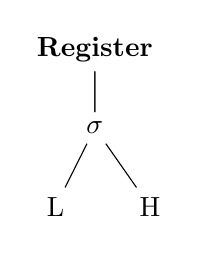
\begin{tikzpicture}	
		\node (tbu) at (.5,0) {\textbf{Register}};
		\node (R) at (.5,-1) {$\sigma$};
		\node (r1) at (0,-2) {L};
		\node (r2) at (1.2,-2) {H};
		\draw (tbu) -> (R) -> (r1);
		\draw (tbu) -> (R) -> (r2);
	\end{tikzpicture}
	\hfill
	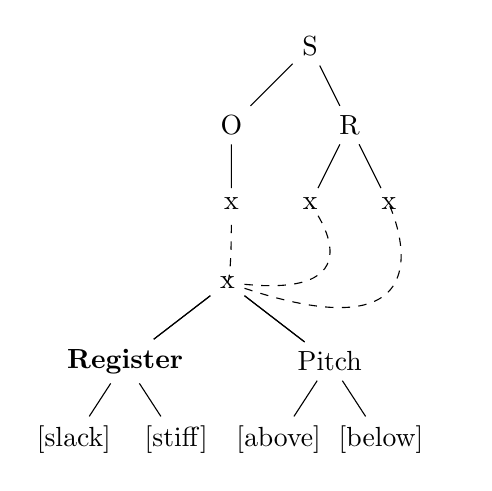
\begin{tikzpicture}
		\node (tbu) at (1.95,0) {x};
		\node (R) at (.65,-1) {\textbf{Register}};
		\node (P) at (3.25,-1) {Pitch};
		\node (r1) at (0,-2) {[slack]};
		\node (r2) at (1.3,-2) {[stiff]};
		\node (p1) at (2.6,-2) {[above]};
		\node (p2) at (3.9,-2) {[below]};
		\draw (tbu) -> (R) -> (r1);
		\draw (tbu) -> (R) -> (r2);
		\draw (tbu) -> (P) -> (p1);
		\draw (tbu) -> (P) -> (p2);
		% Second graph (shifted right)
		\begin{scope}[xshift=3cm, yshift=3cm]
			\node (sS) at (0,0) {S};
			\node (o) at (-1,-1) {O};
			\node (r) at (0.5,-1) {R};
			\node (x1) at (-1,-2) {x};
			\node (x2) at (0,-2) {x};
			\node (x3) at (1,-2) {x};
			\draw (sS) -> (o) -> (x1);
			\draw (sS) -> (r) -> (x2);
			\draw (r) -> (x3);
		\end{scope}
		
		% Cross edges from TBU to Xs
		\draw[dashed] (tbu) .. controls +(0,0) and +(0,-1) .. (x1);
		\draw[dashed] (tbu) .. controls +(2,-0.2) and +(0,0) .. (x2);
		\draw[dashed] (tbu) .. controls +(3,-1) and +(0,0) .. (x3);
	\end{tikzpicture}
	\hfill
	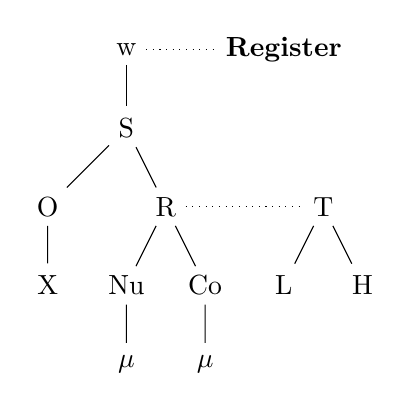
\begin{tikzpicture}[-,shorten >=1pt]
		\tikzstyle{state}=[fill=white,draw=black,text=black,node distance=16mm]
		
		\node (w) at (0,1) {w};
		\node (re) at (2,1) {\textbf{Register}};
		\node (s) at (0,0) {S};
		\node (o) at (-1,-1) {O};
		\node (r) at (0.5,-1) {R};
		\node (T) at (2.5,-1) {T};
		\node (t1) at (2.0,-2) {L};
		\node (t2) at (3,-2) {H};
		
		\node (x1) at (-1,-2) {X};
		\node (x2) at (0,-2) {Nu};
		\node (x3) at (1,-2) {Co};
		\node (m1) at (0,-3) {$\mu$};
		\node (m2) at (1,-3) {$\mu$};
		\draw (w) -> (s);
		\draw (T) -> (t1);
		\draw (T) -> (t2);
		\draw (s) -> (o) -> (x1) ;
		\draw (s) -> (r) -> (x2) -> (m1);
		\draw (r) -> (x3) -> (m2);
		\draw [dotted](r) -> (T);
		\draw [dotted](w) -> (re);
	\end{tikzpicture}
	\label{three-rep}
\end{figure}


\citet{yip1980diss,yip1993tonal} propose that the register should be a feature 
under the tonal node, and also dominate the pitch, as indicated in 
Figure~\ref{three-rep}. Note in Yip's model, the register dominate the pitch 
nodes and apply to each syllable. In polysyllabic forms, only the register
of the inital syllable are retained and the rest are delated. The shortcoming
is that it does not reflect why [+upper] should condition onset voicing. 

Different from \citet{yip1980diss,yip1993tonal}, \citet{duanmu1988} proposed 
that pitch and register are represented on two separate planes: one encodes the 
stiff/slack distinction in voice quality, while the other contains tonal 
features. The motivation is that register is consistently reflected in voice 
quality but not always in pitch. A major difference between Duanmu’s proposal 
and others is that the node represents an X-slot (either a consonant or a 
vowel), and each X-slot is specified for both register and pitch. Consequently, 
whereas a tone can be represented as a single feature bundle in Yip’s system, 
two sets of features are required in Duanmu’s model. For example, [55] is 
represented as [+u, +H] in Yip’s model but as [+st, +H][+st, +H] in Duanmu’s.

Another candidate proposed by \citet{zhu1999shanghai} places register at the 
top of the phonological word, while the pitch node is linked to the rime. This 
differs from Yip’s model in that, whereas Yip connects register to each 
syllable, Zhu’s model assigns a single register node dominating the entire 
word. This accounts for the fact that in polysyllabic words only one register 
value is retained. Unlike the other two models, Zhu’s analysis does not 
associate register with voicing at all.

Another issue in the feature geometry of Shanghainese concerns the 
representation of medial and coda positions. Beyond the placement of register, 
scholars also debate how the syllable should be internally structured. Duanmu 
proposes that all Chinese dialects share the same underlying syllable 
structure. Rather than mora theory, he employs X-slots, positing three slots 
under the syllable node: one for the onset and two for the rime. Zhu, however, 
diverges from this proposal, offering a different analysis of syllable 
structure in Shanghainese.

\section{Proposal}
There are four goals of this paper. First, we would like to compare
In this paper, I compare two competing theories from \citet{duanmu1988}
and \citet{zhu1999shanghai} from a learning perspective. The reason for 
choosing these two models are due the fact that the syllabic structures
that underlie these two models are comparable and clearly porposed, 
the register and pitch nodes can be embeded in at different level of
structure. Besides, these two models are indeed distinct both representationally
and mathmatically. \citet{oakdenNotationalEquivalenceTonal2020} points out
that the long-standing competing theorys between Bao and Yips models are 
in essence equavilent: they do not differet in their empritcal exsirevity 
and they can be translatable into each other without losing nescary contrasts. 
This will be expalined in Section xxx. Each model is represented model-theoretically 
so that all relations within each model, such as association, succession, and dominance, are rigorously captured.



Learning is carried out using the Bottom-Up Factorial Inference Algorithm 
(BUFIA; \citet{chandleeBufia2019}), which operates over model-theoretic inputs 
encoded based on the two models. Our learning goals have two components:

\begin{enumerate}
	\item Tonotactics: the co-occurrence patterns between tones and features\\

	\item Register/voicing assimilation: the rules governing disyllabic compounds.
	
\end{enumerate}

The central question is which representational hypothesis captures the relevant 
generalizations more effectively in tonotactics and register assimilation processes. 
Conversely, if a representation fails to encode the appropriate dependencies, 
the learning resulting over such representation will either overgenerate, 
undergenerate, or produce empirically unattested predictions.




\section{Five Tones in Shanghai}
\begin{table}[h!]
	\centering
	\caption{Phonological features of the five Shanghai tones (\citep{zhu1999shanghai})} 
	\begin{tabular}{lccccc}
		\toprule
		\textbf{Tones} & \textbf{T1} & \textbf{T2} & \textbf{T3} & \textbf{T4} & \textbf{T5} \\
		\midrule
		Register   & +U & +U & -U & +U & -U \\
		Truncation & P  & P  & P  & q  & q  \\
		Contour    & hl & lh & lh & lh & lh \\
		\bottomrule
	\end{tabular}
\end{table}

\bibliography{refs.bib}
\bibliographystyle{apalike}
\end{document}